\section{Disis Iulukinfor}\label{disis-iulukinfor}


\begin{figure}
\centering
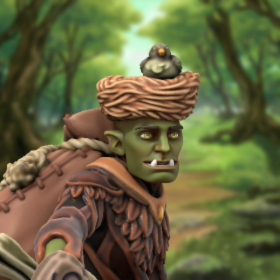
\includegraphics{Disis_Iulukinfor-Token.png}
\caption{Disis Iulukinfor-Token.png}
\end{figure}

Informazioni Generali

Età:

Anno di nascita:

Paese di nascita: Metauros

Razza:

Relazioni:

Alleati:

Nemesi:

Possedimenti importanti:


\subsection{Descrizione Generale}\label{descrizione-generale}


\begin{figure}
\centering
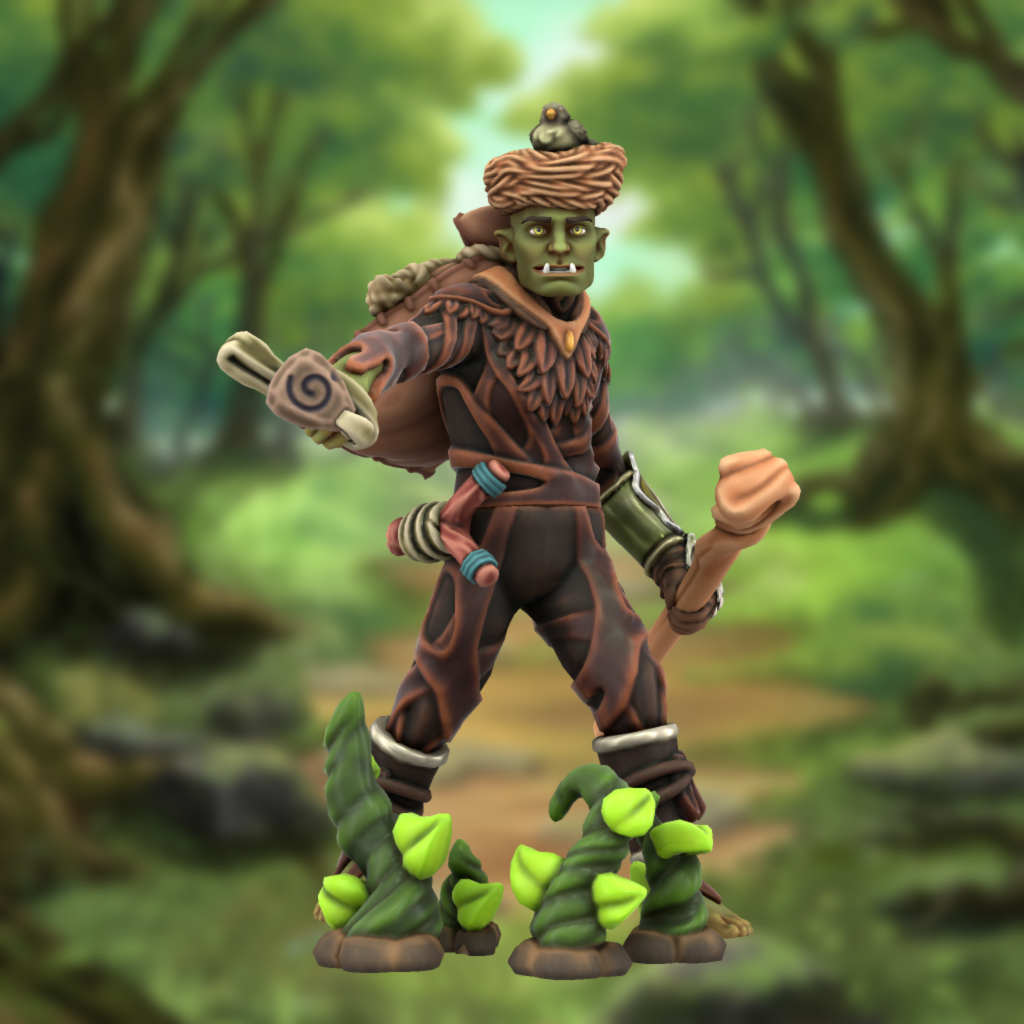
\includegraphics{Disis_Iulukinfor-portrait.png}
\caption{Disis Iulukinfor-portrait.png}
\end{figure}

Disis Iulukinfor è un mezz'orco druido, incarnando l'armonia tra umanità
e natura. La sua pelle abbronzata è attraversata da cicatrici, simboli
del suo passato selvaggio. Gli occhi riflettono saggezza e curiosità,
mentre una chioma corvina incornicia un volto dal fascino unico. Il suo
corpo atletico rivela la profonda connessione con la foresta. Abbigliato
in tonalità terrose, emana un'aura pacifica, trasmettendo sicurezza e un
attaccamento profondo alla natura.

\begin{quote}
``Non sono questi i druidi che state cercando''
\end{quote}

\subsection{Biografia}\label{biografia}


La storia di Disis Iulukinfor inizia con un'origine insolita, nato
dall'incontro tra due mondi, quello umano e quello degli orchi.
Abbandonato poco dopo la nascita nei recessi profondi della foresta,
Disis ebbe la fortuna di essere trovato e adottato dalle creature della
natura. Cresciuto tra animali, spiriti della foresta e creature fatate,
Disis fu avvolto dall'abbraccio amorevole di un ambiente che lo
considerava un proprio figlio. La sua crescita fu segnata
dall'apprendimento dei segreti della natura, dell'arte del druidismo e
della magia che pervadeva gli alberi e le creature stesse. Mentre altri
bambini si familiarizzavano con i confini della società umana, Disis si
immerse nella profonda sapienza delle stagioni, dei venti e degli
animali, diventando un Figlio della Foresta, un protettore e curatore
dell'ambiente che lo aveva accolto. Tuttavia, quando il destino lo portò
a incontrare la civiltà umana, Disis si trovò di fronte a una sfida del
tutto nuova. Confuso e spaesato, si sforzò di adattarsi a usi e costumi
che gli sembravano estranei. La sua capacità di comunicare con gli
animali e il suo cuore gentile gli permisero di stringere amicizie
preziose, aprendo lentamente le porte a un mondo più ampio e complesso.
La sua vita divenne una mescolanza di momenti di contemplazione profonda
nei boschi e di interazioni con le persone che avevano accolto il suo
spirito gentile. Con il tempo, Disis si trasformò in un guardiano della
foresta, un difensore delle creature selvatiche e un portavoce della
natura, cercando di far comprendere agli altri l'importanza di
preservare l'equilibrio dell'ambiente. Liberamente intraprendendo il suo
cammino tra la foresta e le società umane, Disis incarna l'unione di due
mondi e lotta per proteggere l'eredità della foresta che lo ha nutrito,
portando il suo amore per la natura e la sua determinazione a difendere
gli innocenti in ogni angolo del mondo.

\subsection{Carriera}\label{carriera}


La carriera di Disis Iulukinfor non è stata definita da titoli o
posizioni, ma piuttosto da un profondo legame con la natura e il suo
ruolo come guardiano degli equilibri naturali. Fin dalla giovane età,
Disis è stato introdotto alla magia e alla saggezza druidica dalla
foresta stessa. Questa connessione lo ha guidato in un percorso di
apprendimento costante, in cui ha imparato a comunicare con gli animali,
a manipolare le energie naturali e a proteggere l'ambiente circostante.

Inizialmente cresciuto lontano dalla società umana, la sua carriera è
stata forgiata nell'oscurità della foresta, dove ha agito come
intermediario tra le creature selvatiche e gli spiriti della natura. La
sua abilità nel comunicare con gli animali gli ha permesso di sviluppare
un'intesa profonda con le creature che popolano i boschi, facendo di lui
un protettore naturale e un mediatore nei conflitti tra le varie specie.

Con il passare del tempo, il suo ruolo si è espanso, portandolo ad
interagire sempre di più con la società umana. Disis ha iniziato a
condividere la sua conoscenza della natura con coloro che desideravano
ascoltarlo, spiegando l'importanza di rispettare l'ambiente e di
preservare l'equilibrio ecologico. Ha partecipato a iniziative di
conservazione, educando le persone sulle pratiche sostenibili e guidando
escursioni per far conoscere l'ambiente naturale.

La sua carriera non è limitata a un singolo percorso; piuttosto, è un
intreccio di momenti trascorsi nel fitto dei boschi, conversazioni con
creature alate e lezioni impartite su come coesistere in armonia con la
natura. Disis incarna il legame tra l'umanità e il regno naturale,
portando con sé l'eredità del suo passato e la responsabilità del suo
futuro, sempre impegnato a difendere la bellezza e l'equilibrio del
mondo naturale che ama e protegge.

\subsection{Personalità}\label{personalituxe0}


La personalità di Disis Iulukinfor è un intreccio di sfumature,
riflettendo sia l'influenza della natura che la complessità della sua
dualità come mezz'orco. Riservato e riflessivo, Disis porta con sé la
tranquillità dei boschi, un'aura che invita alla contemplazione e al
rispetto. La sua natura tranquilla è un riflesso dell'armonia che cerca
di promuovere nel mondo, facendolo apparire spesso in uno stato di calma
serena.

La sua gentilezza è disarmante, il suo cuore aperto a tutti coloro che
si dimostrano rispettosi e desiderosi di ascoltare le voci della natura.
Con una comunicazione che va al di là delle parole, è in grado di
stabilire connessioni profonde con le creature della foresta, offrendo
amicizia e comprensione dove altri potrebbero vedere solo ferocia.

Sebbene riservato, Disis ha un lato avventuroso e curioso. La sua natura
di Figlio della Foresta lo spinge a esplorare nuovi territori, sia
fisici che emotivi. Questa curiosità lo ha portato a interagire con la
società umana, sfidando le sue ansie e cercando di capire il mondo al di
fuori delle selve.

La sua personalità riflette un profondo rispetto per tutte le forme di
vita. È capace di compassione e di provare dolore per il sofferenza
altrui, ma è altrettanto capace di agire con fermezza quando la natura è
minacciata. La sua determinazione a proteggere l'ambiente naturale e le
creature che vi abitano lo rende un avvocato appassionato per la
conservazione.

In sintesi, Disis è un individuo dalla personalità riflessiva, gentile e
protettiva, ispirato dalla saggezza della natura e determinato a
diffondere armonia e comprensione. La sua personalità è un riflesso del
mondo che abbraccia, un mondo di connessioni profonde e di equilibrio
sottolineato da una passione incrollabile per la conservazione e la
protezione.

